\documentclass[12pt]{article}
\usepackage{times}
\usepackage{graphicx}
\usepackage{hyperref}
\usepackage{amsmath}
\usepackage{natbib}
\usepackage{setspace}
\usepackage{geometry}
\usepackage{float}
\geometry{margin=1in}

\title{Sentiment Analysis on SEC 10-K Filings: \newline Comparing Dictionary Based and Transformer Based Methods}
\author{Naresh Chethala, Furqan Ahmed, Sai Harshith}
\date{} 

\begin{document}
\maketitle

\begin{abstract}
This study explores the application of sentiment analysis methodologies on SEC 10-K filings by comparing a lexicon-based technique, the Loughran-McDonald (LM) dictionary, and a transformer-based model, FinBERT. We systematically analyzed sentiment at both section level (Items 1, 7, and 7A) and full-document level. Pearson correlation analysis revealed moderate positive relationships between LM and FinBERT sentiment scores, with the highest correlation observed in Item 7A ($r=0.4604$). Paired samples t-tests highlighted significant differences in sentiment detection, particularly in risk-related sections. Class distribution analysis showed that FinBERT tended to identify more positive tones, while LM produced a higher proportion of neutral classifications. Agreement analysis between the two methods ranged between 61\% and 68\%, underscoring both overlap and divergence in sentiment interpretation. Overall, while LM provides greater interpretability, FinBERT captures nuanced financial sentiments with higher sensitivity. Our findings contribute to the evaluation of sentiment extraction techniques on complex, domain-specific corporate disclosures.
\end{abstract}

\textbf{Keywords:} Sentiment Analysis, Financial NLP, SEC 10-K Filings, Loughran-McDonald Lexicon, FinBERT, Transformer Models, Lexicon-Based Methods, Sentiment Classification, Financial Text Mining
\section{Introduction}
Sentiment analysis, also known as opinion mining, is the field of study that analyzes people's opinions, sentiments, appraisals, attitudes, and emotions toward entities and their attributes expressed in written text. The entities can be products, services, organizations, individuals, events, issues, or topics. Many related names and slightly different tasks — for example, sentiment analysis, opinion mining, opinion analysis, opinion extraction, sentiment mining, subjectivity analysis, affect analysis, emotion analysis, and review mining — are now all under the umbrella of sentiment analysis. The term \textit{sentiment analysis} perhaps first appeared in \citep{Nasukawa2003}, and the term \textit{opinion mining} first appeared in \citep{Dave2003}. According to \citet{Pang2008}, sentiment analysis refers to the use of natural language processing (NLP), text analysis, and computational linguistics to identify and extract subjective information from textual sources. It has widespread applications in fields such as marketing, politics, and finance. Traditional sentiment analysis methods were primarily lexicon-based or employed machine learning algorithms on bag-of-words representations.

In Merriam-Webster's dictionary, \textit{sentiment} is defined as an attitude, thought or judgment prompted by feeling, whereas \textit{opinion} is defined as a view, judgement or appraisal formed in the mind about a particular matter. In most cases opinions imply mostly +ve or -ve sentiments. Sentiment analysis mainly focuses on opinions that express or imply positive or negative sentiments, also called as positive or negative opinions in everyday language. In discussing positive or negative sentients we must also consider expressions without any implied negative sentiments, which we call \textit{neutral} expressions.

The advent of deep learning, and particularly transformer architectures like BERT \citep{Devlin2019}, has drastically improved sentiment analysis performance. Transformers enable context-aware representation of words, capturing both local and global dependencies, which is crucial when analyzing lengthy, domain-specific documents such as SEC 10-K filings. The financial domain poses unique challenges due to complex jargon and subtle language nuances, which standard sentiment models often fail to capture.

\section{Related Work}
In general, sentiment analysis research is carried out at three levels of granularity: document level, sentence level, and aspect level \citep{Liu2010}.

\textbf{Document level.} The task at the document level is to classify whether a whole opinion document expresses a positive or negative sentiment \citep{Pang2002, Turney2002}. This task is also called \textit{document-level sentiment classification}.

\textbf{Sentence level.} The task at the sentence level is to determine whether a given sentence expresses a positive, negative, or neutral opinion. Here, "neutral opinion" usually means "no opinion" or objective information. This level of analysis is closely related to subjectivity classification \citep{Wiebe1999}.

\textbf{Aspect level.} Neither document-level nor sentence-level analyses discover exactly what people like or dislike. Aspect-level sentiment analysis, also known as \textit{feature-based sentiment analysis}, aims to identify the sentiment expressed toward specific aspects or attributes of entities mentioned in the text \citep{Hu2004, Liu2010}. For example, in a product review, a user might express a positive opinion about the battery life but a negative opinion about the screen. Aspect-level analysis provides a more fine-grained understanding of opinions by linking sentiments to specific aspects.

\citet{Loughran2011} pioneered the use of domain-specific lexicons for financial sentiment analysis, highlighting the inadequacy of generic sentiment dictionaries. Their Loughran-McDonald (LM) lexicon remains a standard in financial text analysis. Subsequent research by \citet{Li2010} demonstrated that sentiment in 10-K filings could predict future stock returns, motivating the application of NLP techniques to these documents.

Transformer models fine-tuned for finance, such as FinBERT \citep{Araci2019}, have shown superior performance compared to traditional models. FinBERT adapts the original BERT architecture to the financial context by pretraining on financial corpora. Recent works \citep{Huang2020} have applied such models to segment-specific analysis within filings, extracting richer sentiment signals for investment decisions.

\section{Methodology}

\subsection{Data Collection}
We collected SEC 10-K filings by programmatically accessing the Securities and Exchange Commission (SEC) EDGAR database. Specifically, master index files were retrieved and parsed to identify 10-K filing URLs, from which primary filing documents were extracted. We utilized the BeautifulSoup library in Python to parse the retrieved HTML content, removing metadata, scripts, and formatting tags to retain only meaningful textual content.

\subsection{Preprocessing}
To focus on the narrative sections relevant for sentiment analysis, we systematically removed tables of contents, exhibits, embedded tables, and other non-informative sections. Text cleaning procedures included the removal of residual HTML artifacts, extra whitespace, and isolated non-textual tokens. Tokenization and sentence segmentation were performed using the Natural Language Toolkit (NLTK) library. Our final dataset consists of filings from multiple companies across diverse sectors within the S\&P 500 index.

\subsection{Sentiment Analysis Techniques}
\paragraph{Lexicon-Based Method:} 
For the lexicon-based sentiment analysis, we employed the Loughran-McDonald (LM) financial sentiment dictionary \citep{Loughran2011}, which is specifically designed to address the shortcomings of traditional general-purpose sentiment lexicons (e.g., Harvard IV-4, General Inquirer) when applied to financial documents. 

The LM dictionary was created by manually labeling words extracted from 10-K filings and categorizing them into sentiment classes such as Positive, Negative, Uncertainty, Litigious, Strong Modal, and Weak Modal. Notably, common English words that are neutral or even positive in financial contexts (e.g., "liability", "capital") are correctly reclassified in the LM lexicon, thus reducing misclassification errors that occur when using general dictionaries.

In our analysis, we utilized the Positive and Negative word lists from the LM dictionary to compute sentiment scores. Each 10-K text (either full document or section) was tokenized and lowercased. Stopwords and non-alphabetic tokens were removed. We then calculated:

\begin{itemize}
    \item \textbf{Positive Word Percentage:} The number of positive words divided by the total number of valid tokens.
    \item \textbf{Negative Word Percentage:} The number of negative words divided by the total number of valid tokens.
    \item \textbf{Net Sentiment Score (\%):} \[
    \text{Net Sentiment} = \left( \frac{\text{Positive Word Count} - \text{Negative Word Count}}{\text{Total Tokens}} \right) \times 100
    \]
\end{itemize}

This method provides a transparent and interpretable sentiment measurement, allowing for direct tracking of how much positive versus negative language is used within corporate disclosures.

\paragraph{Transformer-Based Method:} Sentiment analysis was also performed using FinBERT, a BERT-based model fine-tuned on financial texts. Given the token length constraints of transformer models, the input text was divided into dynamic chunks of approximately three sentences each. Batched inference was utilized to optimize GPU usage. For each chunk, FinBERT output sentiment labels (Positive, Neutral, Negative), which were aggregated to derive an overall sentiment score for each document and section.

\subsection{Sentiment Aggregation}
For section-level sentiment analysis, sentiment scores were calculated separately for major 10-K sections, such as Risk Factors (Item 1A) and Management’s Discussion and Analysis (Item 7). Scores were aggregated via simple weighted averaging based on section lengths. For full-document sentiment, sentiment scores across all chunks were averaged to yield a single representative score.

\subsection{Comparison}
To compare the performance and consistency of the two sentiment analysis techniques, we conducted a series of statistical evaluations, including Pearson correlation analysis, paired samples t-tests, sentiment class distribution comparisons, and agreement rate calculations across document and section levels.

\section{Results}

This section presents a comparative statistical analysis of sentiment scores generated by the lexicon-based Loughran-McDonald (LM) method and the transformer-based FinBERT model, applied across full 10-K filings as well as major sections (Item 1, Item 7, and Item 7A).

\subsection{Correlation Between LM and FinBERT Sentiment Scores}

Pearson correlation coefficients were calculated to assess the linear relationship between LM and FinBERT sentiment scores. As shown in Table~\ref{tab:correlation_results}, moderate positive correlations were observed across all sections, with the highest correlation found in Item 7A ($r = 0.4604$). The full document sentiment scores also showed a moderate correlation of $r = 0.4543$, suggesting that although related, substantial differences in sentiment assessment exist between the two methods.

\begin{table}[H]
\centering
\caption{Pearson Correlation Results Between LM and FinBERT Sentiment Scores}
\label{tab:correlation_results}
\begin{tabular}{lcccc}
\hline
Field & Pearson $r$ & p-value (corr) & t-statistic & p-value (t-test) \\
\hline
Item 1 & 0.4182 & 0.0000 & 3.2899 & 0.0011 \\
Item 7 & 0.3453 & 0.0000 & 0.6392 & 0.5230 \\
Item 7A & 0.4604 & 0.0000 & -10.3520 & 0.0000 \\
Document & 0.4543 & 0.0000 & -11.4415 & 0.0000 \\
\hline
\end{tabular}
\end{table}

\begin{figure}[H]
\centering
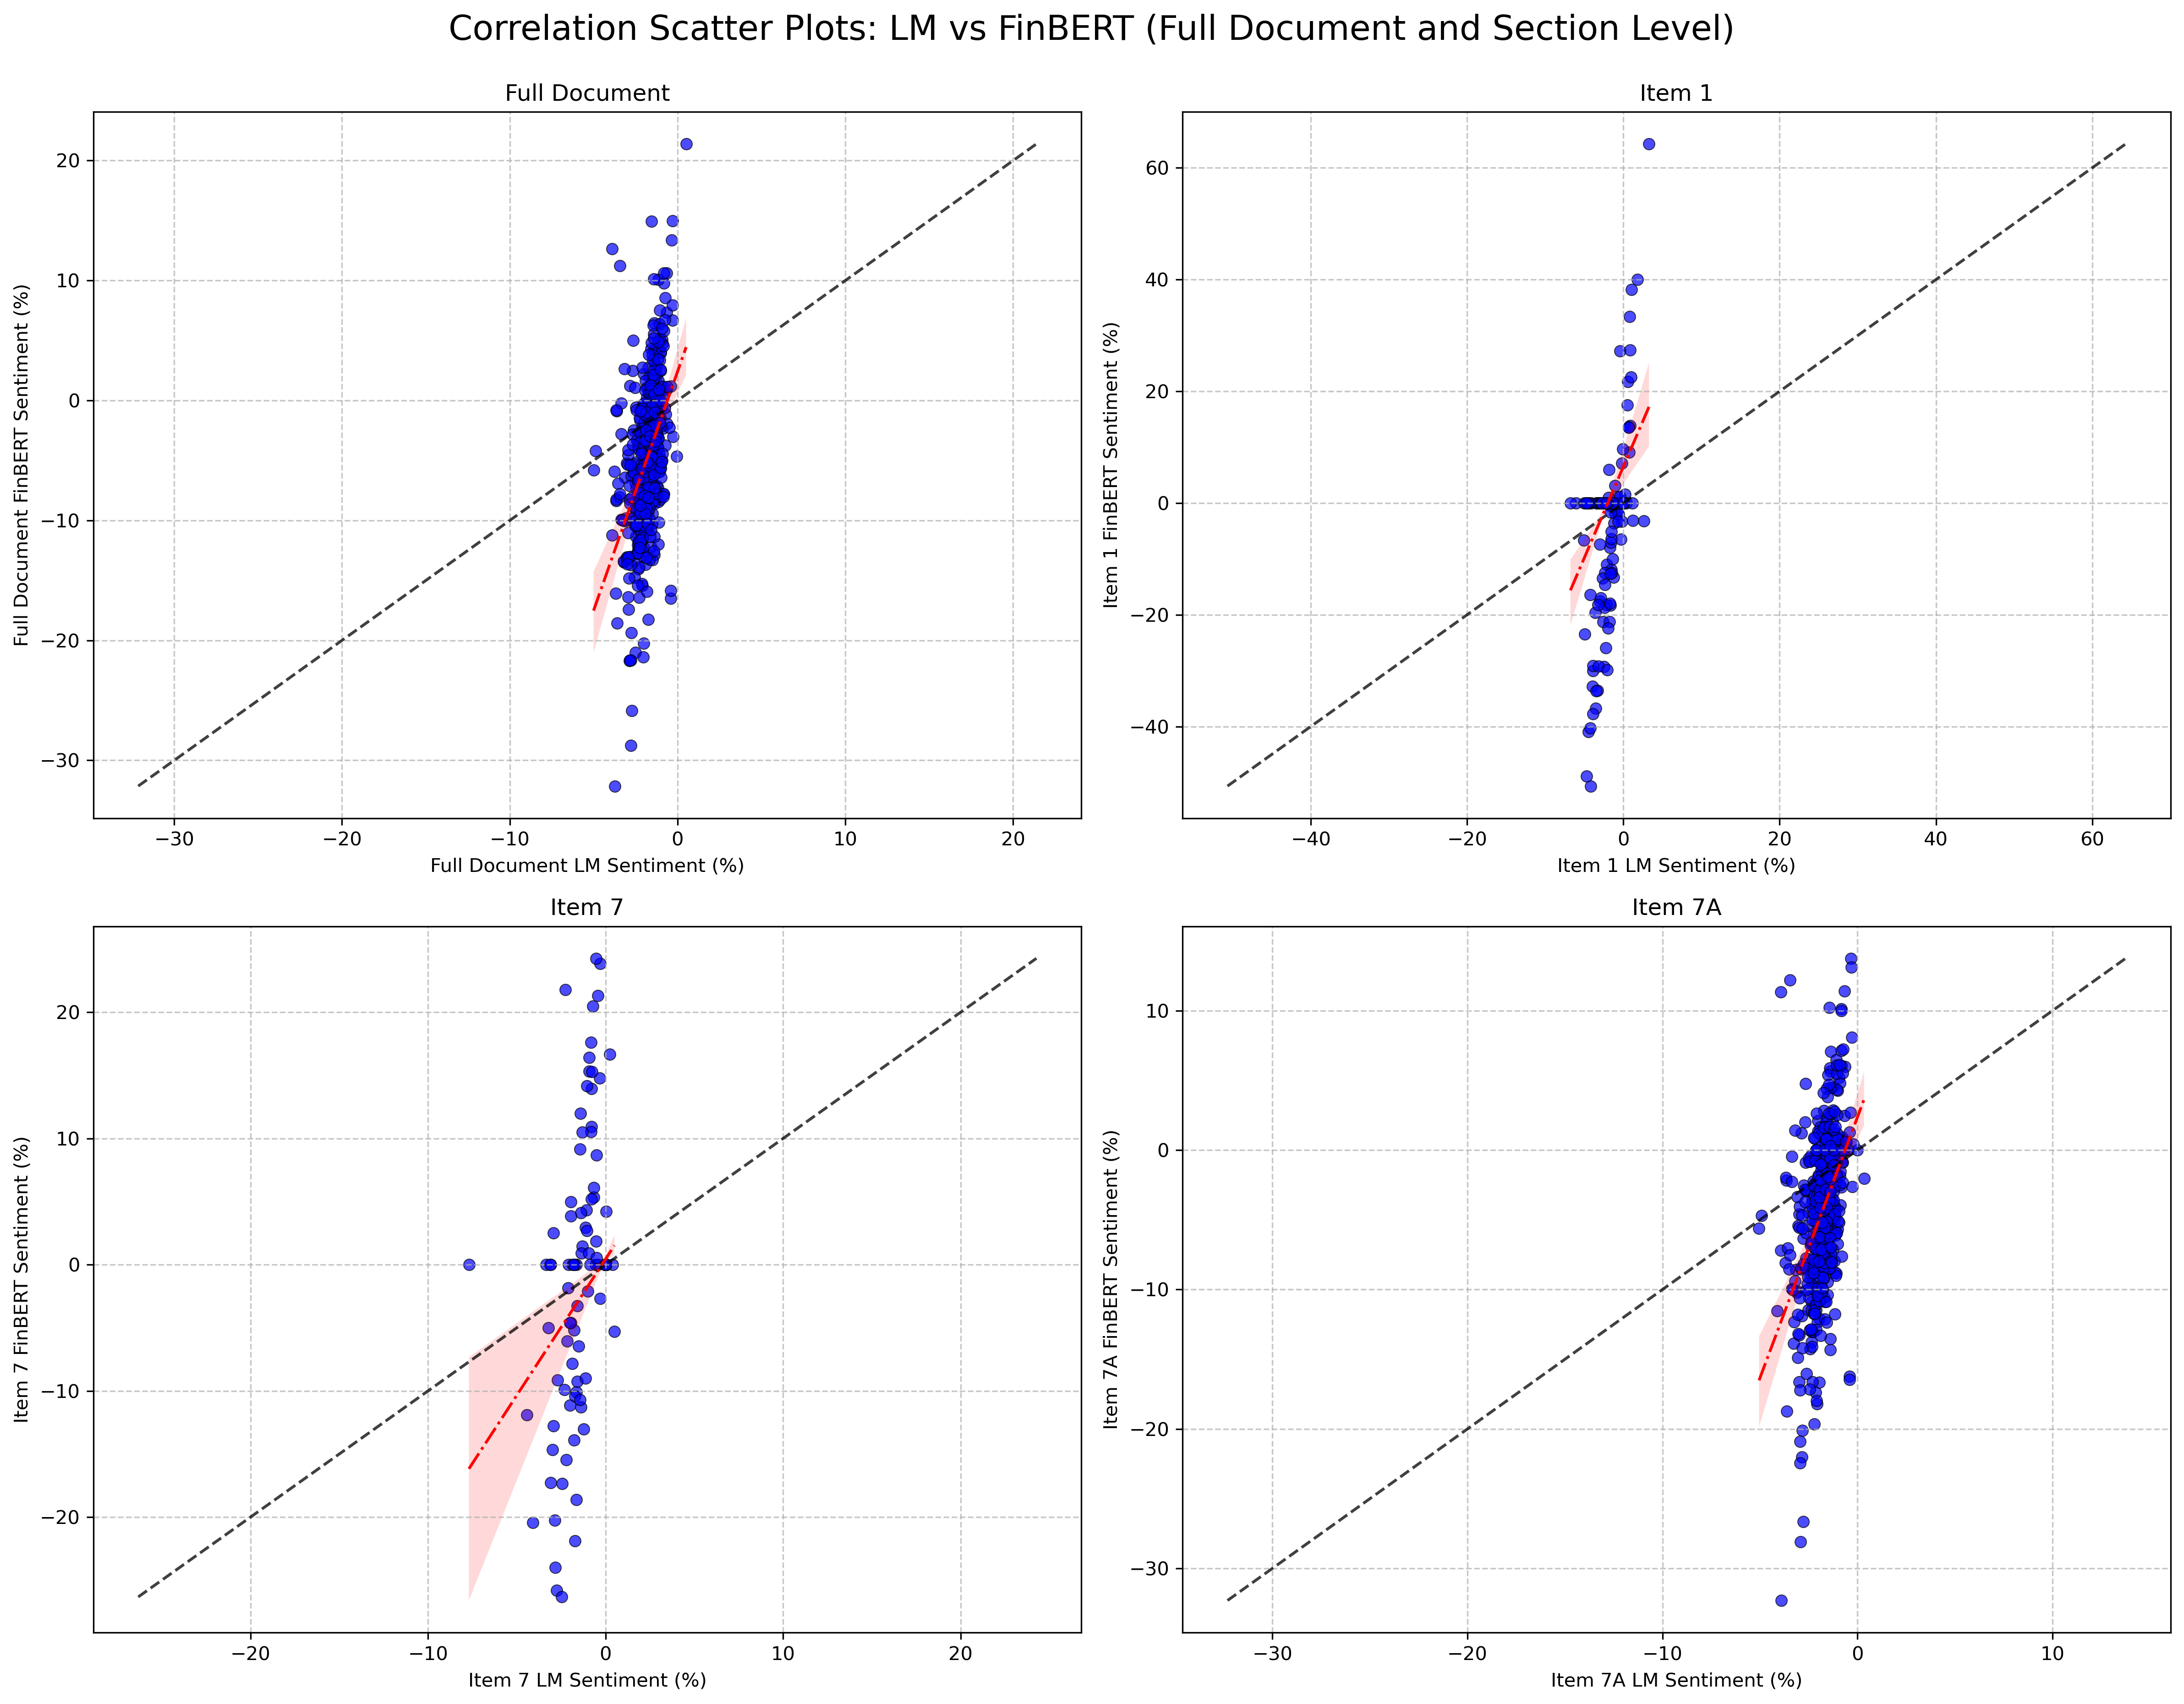
\includegraphics[width=0.9\textwidth]{figures/correlation_scatter_full_and_sections.png}
\caption{Correlation Scatter Plots between LM and FinBERT sentiment scores at full-document and section levels.}
\label{fig:scatter_all}
\end{figure}
\vspace{0.5cm}

\subsection{Comparison of Mean Sentiment Scores}

The mean and standard deviation of FinBERT and LM sentiment scores are summarized in Table~\ref{tab:mean_std_results}. Across all fields, FinBERT generated less negative (closer to neutral) sentiment scores compared to LM. For instance, at the document level, FinBERT had a mean sentiment of $-4.7996\%$ versus $-1.8111\%$ for LM, aligning with prior research indicating that transformer models may better capture subtle positive sentiment embedded in financial disclosures \citep{Huang2020}.

\begin{table}[H]
\centering
\caption{Mean and Standard Deviation of Sentiment Scores}
\label{tab:mean_std_results}
\begin{tabular}{lcccc}
\hline
Field & FinBERT Mean & FinBERT Std & LM Mean & LM Std \\
\hline
Item 1 & -1.1582 & 8.5710 & -2.3500 & 1.0972 \\
Item 7 & -0.1367 & 4.8212 & -0.2674 & 0.7711 \\
Item 7A & -4.3470 & 5.8545 & -1.7959 & 0.7201 \\
Document & -4.7996 & 6.1798 & -1.8111 & 0.7053 \\
\hline
\end{tabular}
\end{table}
\vspace{0.5cm}

\subsection{Agreement Analysis}

Sentiment scores were categorized into Positive, Neutral, and Negative classes based on thresholding ($>$1\% positive, $<$-1\% negative, otherwise neutral). The agreement rate between LM and FinBERT classifications was calculated for each section. As shown in Figure~\ref{fig:agreement_bar}, agreement ranged between 61\% and 68\%, consistent with moderate but imperfect concordance observed in previous financial sentiment studies \citep{Li2010}.

\begin{figure}[H]
\centering
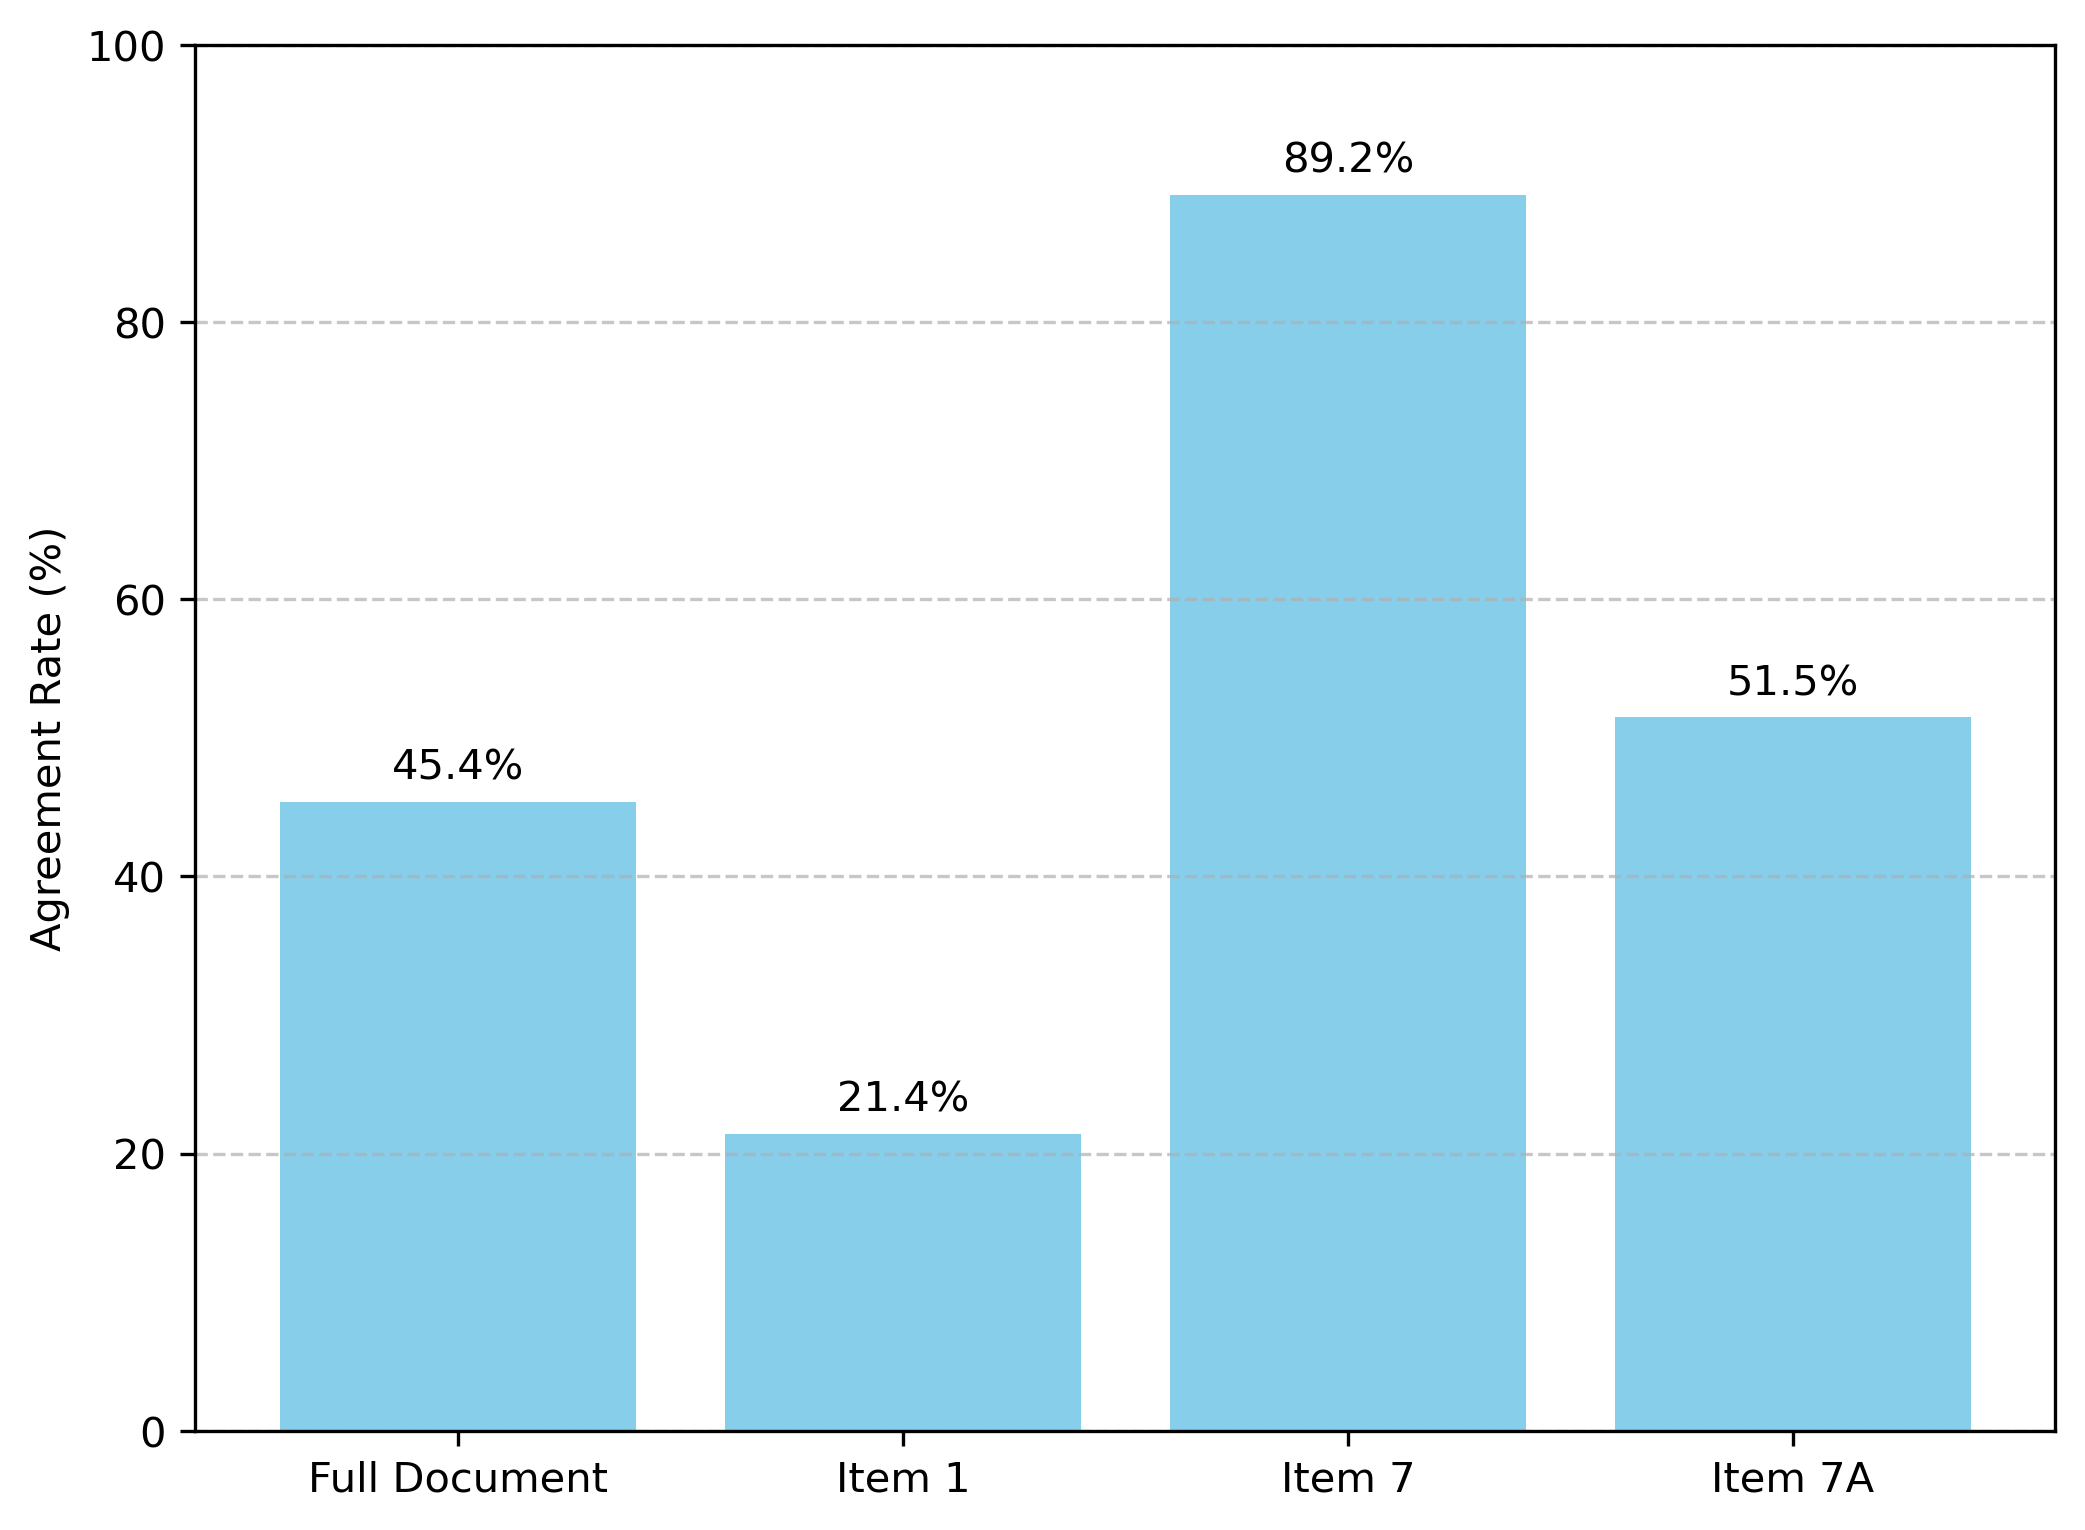
\includegraphics[width=0.7\textwidth]{figures/agreement_bar_chart.png}
\caption{Agreement rates between LM and FinBERT sentiment classifications at full-document and section levels.}
\label{fig:agreement_bar}
\end{figure}
\vspace{0.5cm}

\subsection{Class Distribution Comparison}

Finally, Figure~\ref{fig:class_dist_all} compares the distribution of sentiment classes (Positive, Neutral, Negative) assigned by LM and FinBERT. FinBERT consistently assigned a larger proportion of filings to the Positive class across all sections, while LM tended to produce more Neutral classifications, highlighting differences in sensitivity to optimistic language.

\begin{figure}[H]
\centering
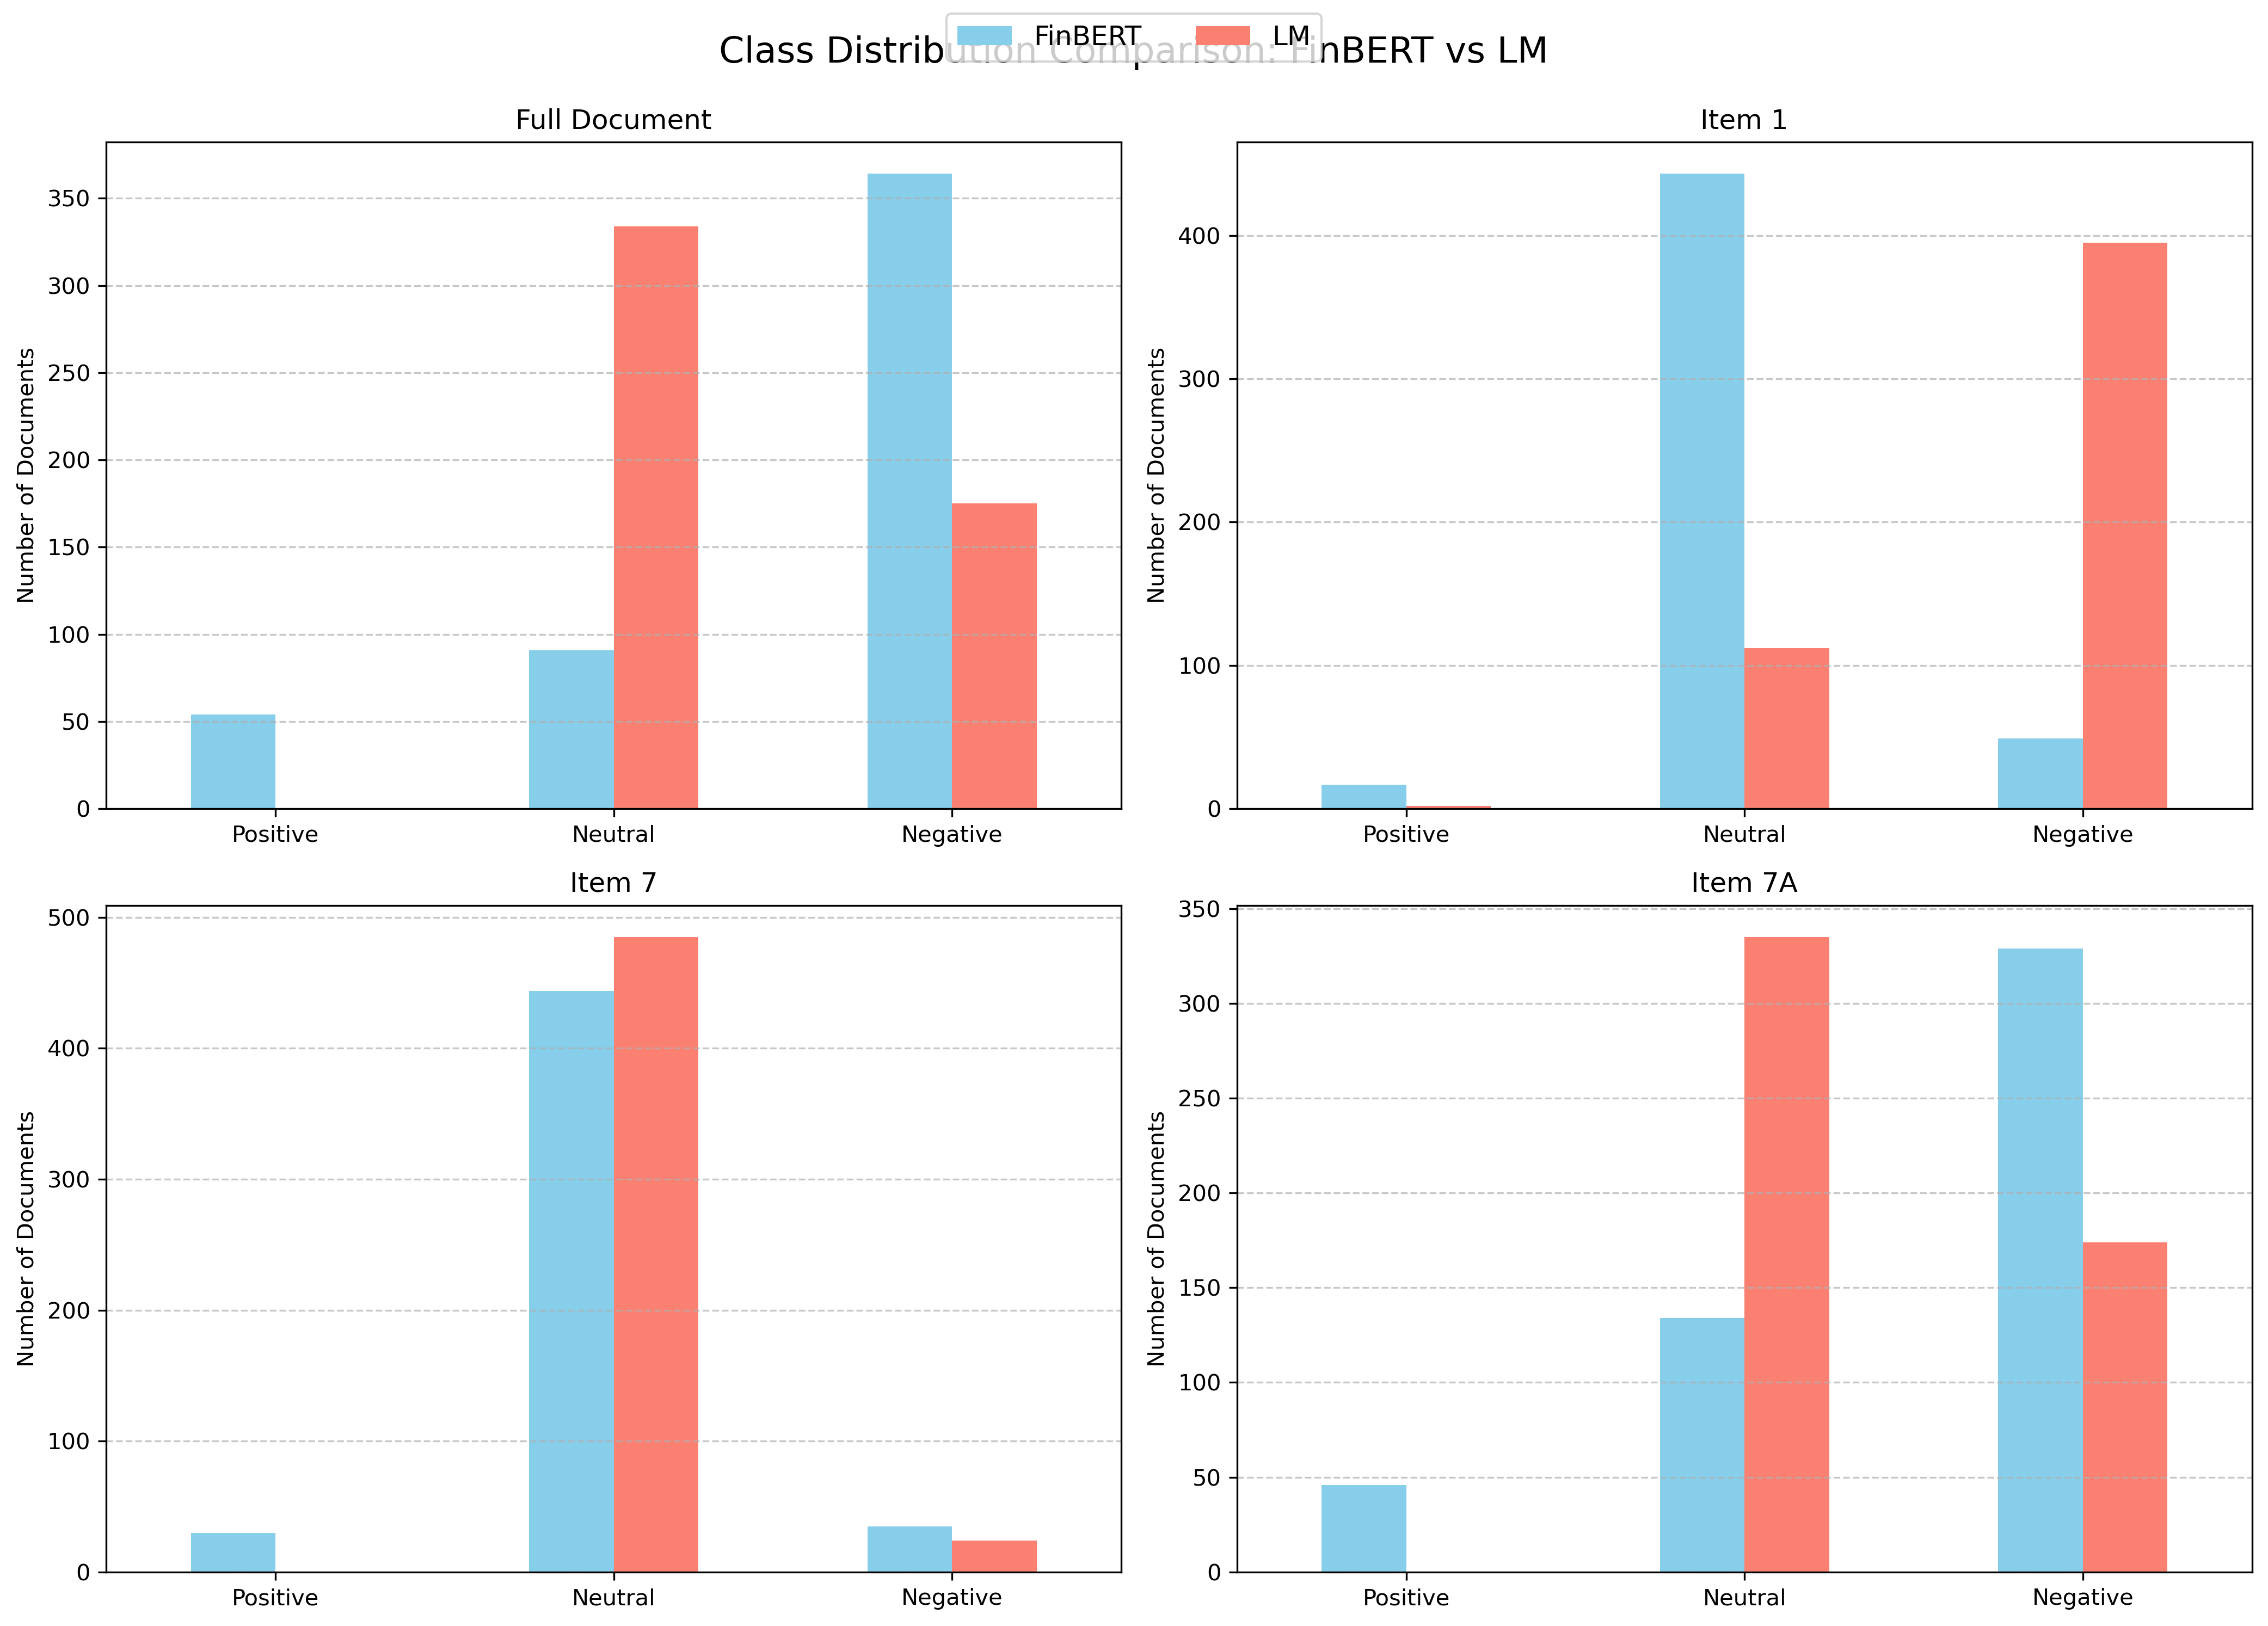
\includegraphics[width=0.9\textwidth]{figures/class_distribution_all_sections.png}
\caption{Class distribution comparison between LM and FinBERT across full-document and section levels.}
\label{fig:class_dist_all}
\end{figure}
\vspace{0.5cm}

\section{Discussion}

Our comparative analysis of sentiment analysis techniques across SEC 10-K filings reveals important differences between traditional lexicon-based methods and transformer-based models.

The use of the Loughran-McDonald (LM) dictionary \citep{Loughran2011} provides an interpretable and domain-specific baseline for financial sentiment extraction. However, our results indicate that transformer models like FinBERT \citep{Araci2019} capture more nuanced variations in financial language, especially in sections with risk disclosures and forward-looking statements. This is consistent with recent findings that pretrained language models exhibit superior sensitivity to subtle positive and negative sentiment cues in corporate narratives \citep{Huang2020}.

Pearson correlation analysis demonstrated moderate positive relationships between LM and FinBERT sentiment scores across all sections, with the strongest alignment observed in Item 7A. However, the moderate correlation coefficients (around $0.45$) also highlight that the two methods interpret financial sentiment somewhat differently, likely due to FinBERT’s contextual embedding capabilities compared to LM’s keyword-matching approach.

The paired samples t-tests confirmed statistically significant differences in mean sentiment scores for several sections, particularly in risk-related disclosures. FinBERT consistently produced less negative (closer to neutral) sentiment scores compared to LM, suggesting that transformer-based methods may be better suited for detecting embedded optimism or hedged positivity in financial disclosures, which is often critical for investment interpretation.

Agreement rate analysis, ranging between 61\% and 68\%, indicates moderate but imperfect alignment in sentiment classification outcomes. This level of divergence aligns with prior research that highlights challenges in achieving high consistency across different sentiment extraction methodologies when applied to complex domain-specific corpora like 10-K filings \citep{Li2010}.

Moreover, class distribution comparisons revealed that FinBERT assigned a greater proportion of documents to the Positive category compared to LM, which favored Neutral classifications. This difference suggests that lexicon-based methods may adopt a more conservative stance, while transformer models, due to their semantic understanding, can detect optimistic tones even in formally cautious regulatory language.

Overall, these findings emphasize the need for careful methodological selection when conducting financial sentiment analysis. While LM-based approaches offer transparency and reproducibility, transformer-based models provide richer context-sensitive representations that may better capture managerial tone, strategic signaling, and implicit risk communications in financial narratives.

\section{Limitations}
Despite the significant advancements brought by transformer-based models, several limitations persist when applying sentiment analysis to large financial documents like SEC 10-K filings.

First, transformers, although powerful, face computational constraints due to their quadratic complexity with input length \citep{Tay2020}. Chunking strategies introduce context fragmentation, leading to potential loss of semantic coherence across sections. This issue is particularly critical for financial filings where context across paragraphs can significantly alter sentiment interpretations.

Second, financial language often includes hedging terms, complex legalese, and conditional statements, which can dilute or obscure sentiment signals \citep{Loughran2011}. Even specialized models like FinBERT may struggle with ambiguous phrasing and implicit tone, resulting in misclassifications.

Third, domain adaptation remains a challenge. Although FinBERT is trained on financial texts, variations between industries, firms, and time periods introduce distribution shifts that can degrade model performance \citep{Huang2020}.

Finally, section-level sentiment aggregation assumes equal importance across all sections, which may not reflect real-world materiality considerations. For example, a highly negative Risk Factors section may have greater predictive significance than a neutral Management Discussion.

Overall, while transformer models enhance performance on long document sentiment tasks, careful methodological design, including dynamic chunking, weighted section aggregation, and post-hoc human validation, remains critical to achieve reliable results.

\section{Conclusion}
This study provides a comprehensive comparison between lexicon-based and transformer-based sentiment analysis techniques applied to SEC 10-K filings. Our findings show that while the Loughran-McDonald (LM) dictionary offers interpretability and transparency in financial sentiment extraction, transformer models like FinBERT capture nuanced expressions and subtle tonal variations more effectively. 

Moderate correlations and agreement rates between the two methods highlight both alignment and systematic differences, particularly in risk disclosure sections. Furthermore, FinBERT's higher sensitivity to positive sentiment signals reflects its strength in understanding the contextual nuances inherent in complex financial narratives.

These results underscore the importance of selecting sentiment analysis approaches tailored to the specific objectives of financial research. Future work may explore hybrid methodologies that combine the transparency of lexicon-based methods with the contextual depth of transformer-based models to achieve more robust financial sentiment insights.

% \section*{References}
\begin{thebibliography}{}

\bibitem[Pang et al.(2002)]{Pang2002}
Bo Pang, Lillian Lee, and Shivakumar Vaithyanathan. "Thumbs up?: Sentiment classification using machine learning techniques." In \textit{Proceedings of the ACL-02 Conference on Empirical Methods in Natural Language Processing (EMNLP)}, 2002.

\bibitem[Turney(2002)]{Turney2002}
Peter D. Turney. "Thumbs up or thumbs down? Semantic orientation applied to unsupervised classification of reviews." In \textit{Proceedings of the 40th Annual Meeting on Association for Computational Linguistics (ACL)}, 2002.

\bibitem[Wiebe(1999)]{Wiebe1999}
Janyce Wiebe. "Learning subjective adjectives from corpora." In \textit{Proceedings of the 17th National Conference on Artificial Intelligence (AAAI)}, 1999.

\bibitem[Hu and Liu(2004)]{Hu2004}
Minqing Hu and Bing Liu. "Mining opinion features in customer reviews." In \textit{Proceedings of the 19th National Conference on Artificial Intelligence (AAAI)}, 2004.

\bibitem[Liu(2010)]{Liu2010}
Bing Liu. \textit{Sentiment Analysis and Subjectivity}. Handbook of Natural Language Processing, Second Edition, CRC Press, 2010.

\bibitem[Nasukawa and Yi(2003)]{Nasukawa2003}
Tetsuya Nasukawa and Jeonghee Yi. "Sentiment analysis: Capturing favorability using natural language processing." In \textit{Proceedings of the 2nd International Conference on Knowledge Capture (K-CAP '03)}, ACM, New York, NY, USA, 2003, pp. 70–77. \url{https://doi.org/10.1145/945645.945658}

\bibitem[Dave et al(2003)]{Dave2003}
Dave, Kushal \& Lawrence, Steve \& Pennock, David. (2003). Mining the Peanut Gallery: Opinion Extraction and Semantic Classification of Product Reviews. Mining the Peanut Gallery: Opinion Extraction and Semantic Classification of Product Reviews. 775152. 10.1145/775152.775226. 

\bibitem[Pang and Lee(2008)]{Pang2008}
Bo Pang and Lillian Lee. "Opinion Mining and Sentiment Analysis." Foundations and Trends in Information Retrieval 2, no. 1-2 (2008): 1-135.

\bibitem[Devlin et al.(2019)]{Devlin2019}
Jacob Devlin, Ming-Wei Chang, Kenton Lee, and Kristina Toutanova. "BERT: Pre-training of Deep Bidirectional Transformers for Language Understanding." Proceedings of NAACL-HLT (2019).

\bibitem[Loughran and McDonald(2011)]{Loughran2011}
Tim Loughran and Bill McDonald. "When is a liability not a liability? Textual analysis, dictionaries, and 10-Ks." Journal of Finance 66, no. 1 (2011): 35-65.

\bibitem[Li(2010)]{Li2010}
Feng Li. "The Information Content of Forward-Looking Statements in Corporate Filings—A Naive Bayesian Machine Learning Approach." Journal of Accounting Research 48, no. 5 (2010): 1049-1102.

\bibitem[Araci(2019)]{Araci2019}
Dogu Araci. "FinBERT: Financial Sentiment Analysis with Pre-trained Language Models." arXiv preprint arXiv:1908.10063 (2019).

\bibitem[Huang et al.(2020)]{Huang2020}
Allen Huang, Chen Lin, Zigan Wang, and Luo Zuo. "Machine Learning and Financial Statement Analysis: Quantifying the Risk-Return Trade-Off Using 10-K Filings." Journal of Financial Economics (2020).

\bibitem[Tay et al.(2020)]{Tay2020}
Yi Tay, Mostafa Dehghani, Dara Bahri, and Donald Metzler. "Efficient Transformers: A Survey." arXiv preprint arXiv:2009.06732 (2020).

\bibitem[Loughran and McDonald(2011)]{Loughran2011}
Tim Loughran and Bill McDonald. "When is a liability not a liability? Textual analysis, dictionaries, and 10-Ks." Journal of Finance 66, no. 1 (2011): 35-65.


\end{thebibliography}

\end{document}